% arara: pdflatex

\documentclass{standalone}
\usepackage{pgfplots}
\pgfplotsset{compat=1.12}
\newcommand{\expnumber}[2]{{#1}\mathrm{e}{#2}}


\begin{document}
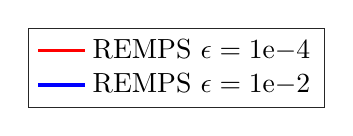
\begin{tikzpicture} 
    \begin{axis}[%
    hide axis,
    xmin=10,
    xmax=50,
    ymin=0,
    ymax=0.4,
    legend style={draw=white!15!black,legend cell align=left}
    ]
    \addlegendimage{red,very thick}
    \addlegendentry{REMPS $\epsilon= \expnumber{1}{-4}$};
    \addlegendimage{blue, very thick}
    \addlegendentry{REMPS $\epsilon= \expnumber{1}{-2}$};
    \end{axis}
\end{tikzpicture}
\end{document}